\documentclass{beamer}

%
% Common preamble for all three parts.
%

\usetheme[block=fill]{metropolis}
\setbeamercolor{frametitle}{use=normal text, parent=normal text}

\usepackage{arevmath}
\SetSymbolFont{largesymbols}{normal}{OMX}{iwona}{m}{n}
\usepackage{fontspec}
\setmainfont{PT Sans}
\setsansfont{PT Sans}
\setmonofont{PT Mono}[Scale=0.87]
\usepackage[english,russian]{babel}
\usepackage{amsmath}
\usepackage{color}
\usepackage{minted}
\usepackage{hyperref}
\usepackage{multicol}
\usepackage{tabularx}
\usepackage{tikz}
\usepackage{tcolorbox}

% For slide 28 (Tikz examples)
\usetikzlibrary{mindmap,trees}
\usetikzlibrary{backgrounds,shapes,arrows,positioning,calc,snakes,fit}
\usepgflibrary{decorations.markings}

\hypersetup{unicode=true}

\tcbuselibrary{skins}
\tcbuselibrary{listings}
\tcbuselibrary{minted}
\tcbset{colframe=mDarkTeal, colback=white!90!mDarkTeal,% Taken from the Metropolis theme
        left=0.8em,right=0.8em}
\newtcolorbox{tblock}[1]{boxsep=1mm,sidebyside=false,bicolor=false,colback=white,title={#1}}
\newtcolorbox{printout}{boxsep=0mm,sidebyside=false,bicolor=false,colback=white}
\def\linkbox#1{\tcbox[on line,boxsep=0mm,left=2pt,right=2pt,top=2pt,bottom=2pt,
                      colback=mDarkTeal,coltext=white]{#1}}
\def\ovllink#1{\tcbox[on line,boxsep=0mm,left=2pt,right=2pt,top=2pt,bottom=2pt,
                      colback=green!30!black,colframe=green!30!black,coltext=white]{#1}}
\newtcblisting{code}{boxsep=0mm,listing only,minted language=latex}
\newtcblisting{bibtexcode}{boxsep=0mm,listing only,minted language=bibtex}
\newtcblisting{exampletwoup}{fontupper=\small,fontlower=\small,
                             boxsep=0mm,listing side text,minted language=latex,
                             bicolor,colbacklower=white,
                             righthand ratio=0.42}
\newtcblisting{exampletwouptiny}{fontupper=\footnotesize,fontlower=\footnotesize,
                                 boxsep=0mm,listing side text,minted language=latex,
                                 minted options={fontsize=\footnotesize},
                                 bicolor,colbacklower=white,
                                 righthand ratio=0.42}
\newtcblisting{exampletwouppaused}{fontupper=\footnotesize,fontlower=\footnotesize,
                             boxsep=0mm,listing side text,minted language=latex,
                             minted options={fontsize=\footnotesize},
                             bicolor,colbacklower=white,
                             righthand ratio=0.42,after lower=\onslide<1->}
\newtcbinputlisting{\inputcode}[2][]{%
listing file={#2},boxsep=0mm,listing only,minted language=latex,#1}
\newtcbinputlisting{\inputbibtexcode}[2][]{%
listing file={#2},boxsep=0mm,listing only,minted language=bibtex,#1}

% only inline todonotes work
\usepackage{xkeyval}
\usepackage[textsize=small]{todonotes}
\presetkeys{todonotes}{inline}{}

\usetikzlibrary{shapes,arrows,positioning,shadows}

% no nav buttons
\usenavigationsymbolstemplate{}

\newcommand{\bftt}[1]{\textbf{\texttt{#1}}}
%\newcommand{\comment}[1]{{\color[HTML]{008080}\textit{\textbf{\texttt{#1}}}}}
\newcommand{\cmd}[1]{{\color[HTML]{008000}\bftt{#1}}}
\newcommand{\bs}{\char`\\}
\newcommand{\cmdbs}[1]{\cmd{\bs#1}}
\newcommand{\lcb}{\char '173}
\newcommand{\rcb}{\char '175}
\newcommand{\cmdbegin}[1]{\cmdbs{begin\lcb}\bftt{#1}\cmd{\rcb}}
\newcommand{\cmdend}[1]{\cmdbs{end\lcb}\bftt{#1}\cmd{\rcb}}

\newcommand{\wllogo}{\textbf{Overleaf}}

% this is where the example source files are loaded from
% do not include a trailing slash
\newcommand{\fileuri}{https://raw.github.com/sgolovan/latex-course/master/ru}

\newcommand{\wlserver}{https://www.overleaf.com}
\newcommand{\wlnewdoc}[1]{\wlserver/docs?snip\_uri=\fileuri/#1\&splash=none}

\def\tikzname{Ti\emph{k}Z}

% from http://tex.stackexchange.com/questions/5226/keyboard-font-for-latex
\newcommand*\keystroke[1]{%
  \tikz[baseline=(key.base)]
    \node[%
      draw,
      fill=white,
      drop shadow={shadow xshift=0.25ex,shadow yshift=-0.25ex,fill=black,opacity=0.75},
      rectangle,
      rounded corners=2pt,
      inner sep=1pt,
      line width=0.5pt,
      font=\scriptsize\ttfamily
    ](key) {#1\strut}
  ;
}
\newcommand{\keystrokebftt}[1]{\keystroke{\bftt{#1}}}

% stolen from minted.dtx
\newenvironment{exampletwouptinynoframe}
  {\VerbatimEnvironment
   \begin{VerbatimOut}{example.out}}
  {\end{VerbatimOut}
   \setlength{\parindent}{0pt}
   \begin{tabular}{l|l}
   \begin{minipage}{0.55\linewidth}
     \inputminted[fontsize=\scriptsize,resetmargins]{latex}{example.out}
   \end{minipage} &
   \begin{minipage}{0.35\linewidth}
     \setlength{\parskip}{6pt plus 1pt minus 1pt}%
     \raggedright\scriptsize\input{example.out}
   \end{minipage}
   \end{tabular}}

\title{Интерактивное введение в \LaTeX}
\author{Джон Д. Лис-Миллер\\Перевод на русский язык: Сергей Головань}
%\titlegraphic{%
%\includegraphics[height=36pt]{overleaf}\\[1em]
%\includegraphics[height=24pt]{UoB-logo}
%}


\subtitle{Часть 1: Основы}

\begin{document}

%%%%%%%%%%%%%%%%%%%%%%%%%%%%%%%%%%%%%%%%%%%%%%%%%%%%%%%%%%%%%%%%%%%%%%%%%%%%%%%
%%%%%%%%%%%%%%%%%%%%%%%%%%%%%%%%%%%%%%%%%%%%%%%%%%%%%%%%%%%%%%%%%%%%%%%%%%%%%%%
%%%%%%%%%%%%%%%%%%%%%%%%%%%%%%%%%%%%%%%%%%%%%%%%%%%%%%%%%%%%%%%%%%%%%%%%%%%%%%%
\begin{frame}
\titlepage
\end{frame}

%%%%%%%%%%%%%%%%%%%%%%%%%%%%%%%%%%%%%%%%%%%%%%%%%%%%%%%%%%%%%%%%%%%%%%%%%%%%%%%
%%%%%%%%%%%%%%%%%%%%%%%%%%%%%%%%%%%%%%%%%%%%%%%%%%%%%%%%%%%%%%%%%%%%%%%%%%%%%%%
%%%%%%%%%%%%%%%%%%%%%%%%%%%%%%%%%%%%%%%%%%%%%%%%%%%%%%%%%%%%%%%%%%%%%%%%%%%%%%%
\begin{frame}{Почему \LaTeX{}?}
\begin{itemize}
\item Он позволяет набирать красивые документы
\begin{itemize}
\item Особенно с математическими формулами
\end{itemize}
%
\item Он был создан учёными для учёных
\begin{itemize}
\item Большое и активное сообщество пользователей и разработчиков
\end{itemize}
%
\item Он мощный, вы можете расширять его
\begin{itemize}
\item Пакеты для статей, презентаций, таблиц, \ldots
\end{itemize}
\end{itemize}
\end{frame}

%%%%%%%%%%%%%%%%%%%%%%%%%%%%%%%%%%%%%%%%%%%%%%%%%%%%%%%%%%%%%%%%%%%%%%%%%%%%%%%
%%%%%%%%%%%%%%%%%%%%%%%%%%%%%%%%%%%%%%%%%%%%%%%%%%%%%%%%%%%%%%%%%%%%%%%%%%%%%%%
%%%%%%%%%%%%%%%%%%%%%%%%%%%%%%%%%%%%%%%%%%%%%%%%%%%%%%%%%%%%%%%%%%%%%%%%%%%%%%%
\begin{frame}[fragile]{Как он работает?}
\begin{itemize}
\item Вы набираете документ в формате \texttt{обычного текста} с \cmd{командами},
  которые описывают его структуру и смысл.
\item Программа \texttt{latex} обрабатывает ваш текст и команды и преобразовывает
  его в красиво отформатированный документ.
\end{itemize}
\vskip 2ex
\begin{center}
\begin{minted}[frame=single]{latex}
Шла Саша по шоссе и сосала \emph{сушку}.
\end{minted}
\vskip 2ex
\tikz\node[single arrow,fill=gray,font=\ttfamily\bfseries,%
  rotate=270,xshift=-1em]{latex};
\vskip 2ex
\fbox{Шла Саша по шоссе и сосала \emph{сушку}.}
\end{center}
\end{frame}

%%%%%%%%%%%%%%%%%%%%%%%%%%%%%%%%%%%%%%%%%%%%%%%%%%%%%%%%%%%%%%%%%%%%%%%%%%%%%%%
%%%%%%%%%%%%%%%%%%%%%%%%%%%%%%%%%%%%%%%%%%%%%%%%%%%%%%%%%%%%%%%%%%%%%%%%%%%%%%%
%%%%%%%%%%%%%%%%%%%%%%%%%%%%%%%%%%%%%%%%%%%%%%%%%%%%%%%%%%%%%%%%%%%%%%%%%%%%%%%
\begin{frame}[fragile]{Ещё примеры команд и их результат\ldots}
\begin{exampletwoup}
\begin{itemize}
\item Чай
\item Молоко
\item Печенье
\end{itemize}
\end{exampletwoup}
\vskip 2ex
\begin{exampletwoup}
\begin{figure}
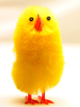
\includegraphics{chick}
\end{figure}
\end{exampletwoup}
\vskip 2ex
\begin{exampletwoup}
\begin{equation}
\alpha + \beta + 1
\end{equation}
\end{exampletwoup}

\tiny{Изображение взято с \url{http://www.andy-roberts.net/writing/latex/importing_images}}
\end{frame}

%%%%%%%%%%%%%%%%%%%%%%%%%%%%%%%%%%%%%%%%%%%%%%%%%%%%%%%%%%%%%%%%%%%%%%%%%%%%%%%
%%%%%%%%%%%%%%%%%%%%%%%%%%%%%%%%%%%%%%%%%%%%%%%%%%%%%%%%%%%%%%%%%%%%%%%%%%%%%%%
%%%%%%%%%%%%%%%%%%%%%%%%%%%%%%%%%%%%%%%%%%%%%%%%%%%%%%%%%%%%%%%%%%%%%%%%%%%%%%%
\begin{frame}[fragile]{Смена подхода}

\begin{itemize}
\item Используйте команды, чтобы описывать <<что это>>, а не <<как это выглядит>>.
\item Сосредоточьтесь на содержании.
\item Позвольте \LaTeX{} делать его работу.
\end{itemize}
\end{frame}

%%%%%%%%%%%%%%%%%%%%%%%%%%%%%%%%%%%%%%%%%%%%%%%%%%%%%%%%%%%%%%%%%%%%%%%%%%%%%%%
%%%%%%%%%%%%%%%%%%%%%%%%%%%%%%%%%%%%%%%%%%%%%%%%%%%%%%%%%%%%%%%%%%%%%%%%%%%%%%%
%%%%%%%%%%%%%%%%%%%%%%%%%%%%%%%%%%%%%%%%%%%%%%%%%%%%%%%%%%%%%%%%%%%%%%%%%%%%%%%
\section{Основы}

%%%%%%%%%%%%%%%%%%%%%%%%%%%%%%%%%%%%%%%%%%%%%%%%%%%%%%%%%%%%%%%%%%%%%%%%%%%%%%%
%%%%%%%%%%%%%%%%%%%%%%%%%%%%%%%%%%%%%%%%%%%%%%%%%%%%%%%%%%%%%%%%%%%%%%%%%%%%%%%
%%%%%%%%%%%%%%%%%%%%%%%%%%%%%%%%%%%%%%%%%%%%%%%%%%%%%%%%%%%%%%%%%%%%%%%%%%%%%%%
\subsection{Первые шаги}
\begin{frame}[fragile]{\insertsubsection}
\begin{itemize}
  \item Минимальный документ \LaTeX{} (на русском языке):

\inputminted[frame=single]{latex}{basics.tex}
\item Команды начинаются с \emph{обратного слэша} \keystrokebftt{\bs}.
\item Каждый документ начинается с команды \cmdbs{documentclass}.
\item \emph{Аргумент} в фигурных скобках \keystrokebftt{\{} \keystrokebftt{\}}
  указывает \LaTeX'у что именно за документ мы пишем: \bftt{article} означает статья.
\item Значок процента \keystrokebftt{\%} начинает \emph{комментарий} --- \LaTeX{}
проигнорирует оставшуюся часть строки.
\end{itemize}
\end{frame}

%%%%%%%%%%%%%%%%%%%%%%%%%%%%%%%%%%%%%%%%%%%%%%%%%%%%%%%%%%%%%%%%%%%%%%%%%%%%%%%
%%%%%%%%%%%%%%%%%%%%%%%%%%%%%%%%%%%%%%%%%%%%%%%%%%%%%%%%%%%%%%%%%%%%%%%%%%%%%%%
%%%%%%%%%%%%%%%%%%%%%%%%%%%%%%%%%%%%%%%%%%%%%%%%%%%%%%%%%%%%%%%%%%%%%%%%%%%%%%%
\begin{frame}[fragile]{\insertsubsection{} в \wllogo}
\begin{itemize}
  \item Overleaf --- это вебсайт, позволяющий набирать документы \LaTeX{} в интернете.
\item Он <<компилирует>> ваш текст \LaTeX{} автоматически и показывает результат.
\vskip 2em
\begin{center}
\fbox{\href{\wlnewdoc{basics.tex}}{%
Щёлкните здесь, чтобы открыть пример в \wllogo{}}}
\\[1ex]\scriptsize{}
Для лучшего результата воспользуйтесь браузером
\href{http://www.google.com/chrome}{Google Chrome} или новой версией браузера
\href{http://www.mozilla.org/en-US/firefox/new/}{FireFox}.
\end{center}
\vskip 2ex
\item В дальнейшем при просмотре сладов пробуйте As we go through the following slides, try out the examples by typing them
into the example document on Overleaf.
\item \textbf{Нет, правда, вы должны их попробовать по мере просмотра!}
\end{itemize}
\end{frame}

%%%%%%%%%%%%%%%%%%%%%%%%%%%%%%%%%%%%%%%%%%%%%%%%%%%%%%%%%%%%%%%%%%%%%%%%%%%%%%%
%%%%%%%%%%%%%%%%%%%%%%%%%%%%%%%%%%%%%%%%%%%%%%%%%%%%%%%%%%%%%%%%%%%%%%%%%%%%%%%
%%%%%%%%%%%%%%%%%%%%%%%%%%%%%%%%%%%%%%%%%%%%%%%%%%%%%%%%%%%%%%%%%%%%%%%%%%%%%%%
\subsection{Набор текста}
\begin{frame}[fragile]{\insertsubsection{}}
\small
\begin{itemize}
\item Набирайте ваш текст между \cmdbegin{document} и \cmdend{document}.
\item По большей части вы можете просто вводить текст как есть.

\begin{exampletwouptiny}
Слова разделяются одним или больше
пробелами.

Абзацы разделяются одной или больше
пустых строк.
\end{exampletwouptiny}
\item Несколько пробелов подряд в исходном тексте воспринимаются как один.

\begin{exampletwouptiny}
Шла     Саша    по  шоссе
и      сосала      сушку.
\end{exampletwouptiny}
\end{itemize}
\end{frame}

%%%%%%%%%%%%%%%%%%%%%%%%%%%%%%%%%%%%%%%%%%%%%%%%%%%%%%%%%%%%%%%%%%%%%%%%%%%%%%%
%%%%%%%%%%%%%%%%%%%%%%%%%%%%%%%%%%%%%%%%%%%%%%%%%%%%%%%%%%%%%%%%%%%%%%%%%%%%%%%
%%%%%%%%%%%%%%%%%%%%%%%%%%%%%%%%%%%%%%%%%%%%%%%%%%%%%%%%%%%%%%%%%%%%%%%%%%%%%%%
\begin{frame}[fragile]{\insertsubsection{}: особенности}
\small
\begin{itemize}
\item Символы кавычек вводятся хитро: используются символы \keystroke{<} и
  \keystroke{>} для <<ёлочек>>, и запятая \keystroke{,} с обратной кавычкой
  \keystroke{\char96} для ,,лапок``.

\begin{exampletwouptiny}
Кавычки-ёлочки: <<текст>>.

Кавычки-лапки: ,,текст``.
\end{exampletwouptiny}

\item Некоторые часто встречающиеся символы имеют специальный смысл в \LaTeX:

\begin{tabular}{cl}
\keystrokebftt{\%} & значок процента     \\
\keystrokebftt{\#} & значок диеза / хэша \\
\keystrokebftt{\&} & амперсанд           \\
\keystrokebftt{\$} & значок доллара      \\
\end{tabular}
\item Если ввести эти символы непосредственно, то получится ошибка. Если
  нужно, чтобы эти значки появились в документе, то их придётся \emph{экранировать}
  с помощью обратного слэша.
\begin{exampletwoup}
\$\%\&\#!
\end{exampletwoup}
\end{itemize}
\end{frame}

%%%%%%%%%%%%%%%%%%%%%%%%%%%%%%%%%%%%%%%%%%%%%%%%%%%%%%%%%%%%%%%%%%%%%%%%%%%%%%%
%%%%%%%%%%%%%%%%%%%%%%%%%%%%%%%%%%%%%%%%%%%%%%%%%%%%%%%%%%%%%%%%%%%%%%%%%%%%%%%
%%%%%%%%%%%%%%%%%%%%%%%%%%%%%%%%%%%%%%%%%%%%%%%%%%%%%%%%%%%%%%%%%%%%%%%%%%%%%%%
\begin{frame}[fragile]{Handling Errors}
\begin{itemize}
\item \LaTeX{} can get confused when it is trying to compile your document. If
it does, it stops with an error, which you must fix before it will produce
any output.
\item For example, if you misspell \cmdbs{emph} as \cmdbs{meph}, \LaTeX{} will
stop with an ``undefined control sequence'' error, because ``meph'' is not
one of the commands it knows.
\end{itemize}
\begin{block}{Advice on Errors}
\begin{enumerate}
\item Don't panic! Errors happen.
\item Fix them as soon as they arise --- if what you just typed caused an error,
you can start your debugging there.
\item If there are multiple errors, start with the first one --- the cause may
even be above it.
\end{enumerate}
\end{block}
\end{frame}

%%%%%%%%%%%%%%%%%%%%%%%%%%%%%%%%%%%%%%%%%%%%%%%%%%%%%%%%%%%%%%%%%%%%%%%%%%%%%%%
%%%%%%%%%%%%%%%%%%%%%%%%%%%%%%%%%%%%%%%%%%%%%%%%%%%%%%%%%%%%%%%%%%%%%%%%%%%%%%%
%%%%%%%%%%%%%%%%%%%%%%%%%%%%%%%%%%%%%%%%%%%%%%%%%%%%%%%%%%%%%%%%%%%%%%%%%%%%%%%
\begin{frame}[fragile]{Typesetting Exercise 1}

\begin{block}{Typeset this in \LaTeX:
\footnote{\url{http://en.wikipedia.org/wiki/Economy_of_the_United_States}}}
In March 2006, Congress raised that ceiling an additional \$0.79 trillion to
\$8.97 trillion, which is approximately 68\% of GDP. As of October 4, 2008, the
``Emergency Economic Stabilization Act of 2008'' raised the current debt ceiling
to \$11.3 trillion.
\end{block}
\vskip 2ex
\begin{center}
\fbox{\href{\wlnewdoc{basics-exercise-1.tex}}{%
Click to open this exercise in \wllogo{}}}
\end{center}

\begin{itemize}
\item Hint: watch out for characters with special meanings!
\item Once you've tried,
\fbox{\href{\wlnewdoc{basics-exercise-1-solution.tex}}{%
click here to see my solution}}.
\end{itemize}
\end{frame}

%%%%%%%%%%%%%%%%%%%%%%%%%%%%%%%%%%%%%%%%%%%%%%%%%%%%%%%%%%%%%%%%%%%%%%%%%%%%%%%
%%%%%%%%%%%%%%%%%%%%%%%%%%%%%%%%%%%%%%%%%%%%%%%%%%%%%%%%%%%%%%%%%%%%%%%%%%%%%%%
%%%%%%%%%%%%%%%%%%%%%%%%%%%%%%%%%%%%%%%%%%%%%%%%%%%%%%%%%%%%%%%%%%%%%%%%%%%%%%%
\subsection{Typesetting Mathematics}
\begin{frame}[fragile]{\insertsubsection{}: Dollar Signs}
\begin{itemize}
\item Why are dollar signs \keystrokebftt{\$} special? We use them to mark mathematics in text.\\[1ex]
\begin{exampletwouptiny}
% not so good:
Let a and b be distinct positive
integers, and let c = a - b + 1.

% much better:
Let $a$ and $b$ be distinct positive
integers, and let $c = a - b + 1$.
\end{exampletwouptiny}
\item Always use dollar signs in pairs --- one to begin the mathematics, and one
to end it.
\item \LaTeX{} handles spacing automatically; it ignores your spaces.
\begin{exampletwouptiny}
Let $y=mx+b$ be \ldots

Let $y = m x + b$ be \ldots
\end{exampletwouptiny}
\end{itemize}
\end{frame}

%%%%%%%%%%%%%%%%%%%%%%%%%%%%%%%%%%%%%%%%%%%%%%%%%%%%%%%%%%%%%%%%%%%%%%%%%%%%%%%
%%%%%%%%%%%%%%%%%%%%%%%%%%%%%%%%%%%%%%%%%%%%%%%%%%%%%%%%%%%%%%%%%%%%%%%%%%%%%%%
%%%%%%%%%%%%%%%%%%%%%%%%%%%%%%%%%%%%%%%%%%%%%%%%%%%%%%%%%%%%%%%%%%%%%%%%%%%%%%%
\begin{frame}[fragile]{\insertsubsection{}: Notation}
\begin{itemize}
\item Use caret \keystrokebftt{\char94} for superscripts and underscore \keystrokebftt{\_} for subscripts.
\begin{exampletwouptiny}
$y = c_2 x^2 + c_1 x + c_0$
\end{exampletwouptiny}
\vskip 2ex

\item Use curly braces \keystrokebftt{\{} \keystrokebftt{\}} to group
superscripts and subscripts.
\begin{exampletwouptiny}
$F_n = F_n-1 + F_n-2$     % oops!

$F_n = F_{n-1} + F_{n-2}$ % ok!
\end{exampletwouptiny}
\vskip 2ex

\item There are commands for Greek letters and common notation.
\begin{exampletwouptiny}
$\mu = A e^{Q/RT}$

$\Omega = \sum_{k=1}^{n} \omega_k$
\end{exampletwouptiny}
\end{itemize}
\end{frame}

%%%%%%%%%%%%%%%%%%%%%%%%%%%%%%%%%%%%%%%%%%%%%%%%%%%%%%%%%%%%%%%%%%%%%%%%%%%%%%%
%%%%%%%%%%%%%%%%%%%%%%%%%%%%%%%%%%%%%%%%%%%%%%%%%%%%%%%%%%%%%%%%%%%%%%%%%%%%%%%
%%%%%%%%%%%%%%%%%%%%%%%%%%%%%%%%%%%%%%%%%%%%%%%%%%%%%%%%%%%%%%%%%%%%%%%%%%%%%%%
\begin{frame}[fragile]{\insertsubsection{}: Displayed Equations}
\begin{itemize}
\item If it's big and scary, \emph{display} it on its own line using
\cmdbegin{equation} and \cmdend{equation}.\\[2ex]
\begin{exampletwouptiny}
The roots of a quadratic equation
are given by
\begin{equation}
x = \frac{-b \pm \sqrt{b^2 - 4ac}}
         {2a}
\end{equation}
where $a$, $b$ and $c$ are \ldots
\end{exampletwouptiny}
\vskip 1em
{\scriptsize Caution: \LaTeX{} mostly ignores your spaces in mathematics, but it
can't handle blank lines in equations --- don't put blank lines in your
mathematics.}
\end{itemize}
\end{frame}

%%%%%%%%%%%%%%%%%%%%%%%%%%%%%%%%%%%%%%%%%%%%%%%%%%%%%%%%%%%%%%%%%%%%%%%%%%%%%%%
%%%%%%%%%%%%%%%%%%%%%%%%%%%%%%%%%%%%%%%%%%%%%%%%%%%%%%%%%%%%%%%%%%%%%%%%%%%%%%%
%%%%%%%%%%%%%%%%%%%%%%%%%%%%%%%%%%%%%%%%%%%%%%%%%%%%%%%%%%%%%%%%%%%%%%%%%%%%%%%
\begin{frame}[fragile]{Interlude: Environments}
\begin{itemize}
\item \bftt{equation} is an \emph{environment} --- a context.
\item A command can produce different output in different contexts.
\begin{exampletwouptiny}
We can write
$ \Omega = \sum_{k=1}^{n} \omega_k $
in text, or we can write
\begin{equation}
  \Omega = \sum_{k=1}^{n} \omega_k
\end{equation}
to display it.
\end{exampletwouptiny}
\vskip 2ex
\item Note how the $\Sigma$ is bigger in the \bftt{equation} environment, and
how the subscripts and superscripts change position, even though we used the
same commands.
\vskip 1em
{\scriptsize In fact, we could have written \bftt{\$...\$} as
\cmdbegin{math}\bftt{...}\cmdend{math}.}
\end{itemize}
\end{frame}

%%%%%%%%%%%%%%%%%%%%%%%%%%%%%%%%%%%%%%%%%%%%%%%%%%%%%%%%%%%%%%%%%%%%%%%%%%%%%%%
%%%%%%%%%%%%%%%%%%%%%%%%%%%%%%%%%%%%%%%%%%%%%%%%%%%%%%%%%%%%%%%%%%%%%%%%%%%%%%%
%%%%%%%%%%%%%%%%%%%%%%%%%%%%%%%%%%%%%%%%%%%%%%%%%%%%%%%%%%%%%%%%%%%%%%%%%%%%%%%
\begin{frame}[fragile]{Interlude: Environments}
\begin{itemize}
\item The \cmdbs{begin} and \cmdbs{end} commands are used to create many
different environments.
\vskip 2ex

\item The \bftt{itemize} and \bftt{enumerate} environments generate lists.
\begin{exampletwouptiny}
\begin{itemize} % for bullet points
\item Biscuits
\item Tea
\end{itemize}

\begin{enumerate} % for numbers
\item Biscuits
\item Tea
\end{enumerate}
\end{exampletwouptiny}
\end{itemize}
\end{frame}

%%%%%%%%%%%%%%%%%%%%%%%%%%%%%%%%%%%%%%%%%%%%%%%%%%%%%%%%%%%%%%%%%%%%%%%%%%%%%%%
%%%%%%%%%%%%%%%%%%%%%%%%%%%%%%%%%%%%%%%%%%%%%%%%%%%%%%%%%%%%%%%%%%%%%%%%%%%%%%%
%%%%%%%%%%%%%%%%%%%%%%%%%%%%%%%%%%%%%%%%%%%%%%%%%%%%%%%%%%%%%%%%%%%%%%%%%%%%%%%
\begin{frame}[fragile]{Interlude: Packages}

\begin{itemize}
\item All of the commands and environments we've used so far are built into
\LaTeX.

\item \emph{Packages} are libraries of extra commands and environments. There
are thousands of freely available packages.

\item We have to load each of the packages we want to use with a
\cmdbs{usepackage} command in the \emph{preamble}.

\item Example: \bftt{amsmath} from the American Mathematical Society.
\begin{minted}[fontsize=\small,frame=single]{latex}
\documentclass{article}
\usepackage{amsmath} % preamble
\begin{document}
% now we can use commands from amsmath here...
\end{document}
\end{minted}
\end{itemize}
\end{frame}

%%%%%%%%%%%%%%%%%%%%%%%%%%%%%%%%%%%%%%%%%%%%%%%%%%%%%%%%%%%%%%%%%%%%%%%%%%%%%%%
%%%%%%%%%%%%%%%%%%%%%%%%%%%%%%%%%%%%%%%%%%%%%%%%%%%%%%%%%%%%%%%%%%%%%%%%%%%%%%%
%%%%%%%%%%%%%%%%%%%%%%%%%%%%%%%%%%%%%%%%%%%%%%%%%%%%%%%%%%%%%%%%%%%%%%%%%%%%%%%
\begin{frame}[fragile]{\insertsubsection{}: Examples with \bftt{amsmath}}
\begin{itemize}
\item Use \bftt{equation*} (``equation-star'') for unnumbered equations.
\begin{exampletwouptiny}
\begin{equation*}
  \Omega = \sum_{k=1}^{n} \omega_k
\end{equation*}
\end{exampletwouptiny}
\item \LaTeX{} treats adjacent letters as variables multiplied together, which
is not always what you want. \bftt{amsmath} defines commands for many common
mathematical operators.
\begin{exampletwouptiny}
\begin{equation*} % bad!
 min_{x,y} (1-x)^2 + 100(y-x^2)^2
\end{equation*}
\begin{equation*} % good!
\min_{x,y}{(1-x)^2 + 100(y-x^2)^2}
\end{equation*}
\end{exampletwouptiny}
\item You can use \cmdbs{operatorname} for others.
\begin{exampletwouptiny}
\begin{equation*}
\beta_i =
\frac{\operatorname{Cov}(R_i, R_m)}
     {\operatorname{Var}(R_m)}
\end{equation*}
\end{exampletwouptiny}
\end{itemize}
\end{frame}

%%%%%%%%%%%%%%%%%%%%%%%%%%%%%%%%%%%%%%%%%%%%%%%%%%%%%%%%%%%%%%%%%%%%%%%%%%%%%%%
%%%%%%%%%%%%%%%%%%%%%%%%%%%%%%%%%%%%%%%%%%%%%%%%%%%%%%%%%%%%%%%%%%%%%%%%%%%%%%%
%%%%%%%%%%%%%%%%%%%%%%%%%%%%%%%%%%%%%%%%%%%%%%%%%%%%%%%%%%%%%%%%%%%%%%%%%%%%%%%
\begin{frame}[fragile]{\insertsubsection{}: Examples with \bftt{amsmath}}
\begin{itemize}{\small
\item Align a sequence of equations at the equals sign
\begin{align*}
(x+1)^3 &= (x+1)(x+1)(x+1) \\
        &= (x+1)(x^2 + 2x + 1) \\
        &= x^3 + 3x^2 + 3x + 1
\end{align*}
with the \bftt{align*} environment.

% for whatever reason, this doesn't play well with the twoup environment
\begin{minted}[fontsize=\small,frame=single]{latex}
\begin{align*}
(x+1)^3 &= (x+1)(x+1)(x+1) \\
        &= (x+1)(x^2 + 2x + 1) \\
        &= x^3 + 3x^2 + 3x + 1
\end{align*}
\end{minted}
\item An ampersand \keystrokebftt{\&} separates the left column (before the
$=$) from the right column (after the $=$).
\item A double backslash \keystrokebftt{\bs}\keystrokebftt{\bs} starts a new
line.
}\end{itemize}
\end{frame}


%%%%%%%%%%%%%%%%%%%%%%%%%%%%%%%%%%%%%%%%%%%%%%%%%%%%%%%%%%%%%%%%%%%%%%%%%%%%%%%
%%%%%%%%%%%%%%%%%%%%%%%%%%%%%%%%%%%%%%%%%%%%%%%%%%%%%%%%%%%%%%%%%%%%%%%%%%%%%%%
%%%%%%%%%%%%%%%%%%%%%%%%%%%%%%%%%%%%%%%%%%%%%%%%%%%%%%%%%%%%%%%%%%%%%%%%%%%%%%%
\begin{frame}[fragile]{Typesetting Exercise 2}

\begin{block}{Typeset this in \LaTeX:}
Let $X_1, X_2, \ldots, X_n$ be a sequence of independent and identically
distributed random variables with $\operatorname{E}[X_i] = \mu$ and
$\operatorname{Var}[X_i] = \sigma^2 < \infty$, and let
\begin{equation*}
S_n = \frac{1}{n}\sum_{i}^{n} X_i
\end{equation*}
denote their mean. Then as $n$ approaches infinity, the random variables
$\sqrt{n}(S_n - \mu)$ converge in distribution to a normal $N(0, \sigma^2)$.
\end{block}
\vskip 2ex
\begin{center}
\fbox{\href{\wlnewdoc{basics-exercise-2.tex}}{%
Click to open this exercise in \wllogo{}}}
\end{center}
\begin{itemize}
\item Hint: the command for $\infty$ is \cmdbs{infty}.
\item Once you've tried,
\fbox{\href{\wlnewdoc{basics-exercise-2-solution.tex}}{%
click here to see my solution}}.
\end{itemize}
\end{frame}

%%%%%%%%%%%%%%%%%%%%%%%%%%%%%%%%%%%%%%%%%%%%%%%%%%%%%%%%%%%%%%%%%%%%%%%%%%%%%%%
%%%%%%%%%%%%%%%%%%%%%%%%%%%%%%%%%%%%%%%%%%%%%%%%%%%%%%%%%%%%%%%%%%%%%%%%%%%%%%%
%%%%%%%%%%%%%%%%%%%%%%%%%%%%%%%%%%%%%%%%%%%%%%%%%%%%%%%%%%%%%%%%%%%%%%%%%%%%%%%
\begin{frame}{End of Part 1}
\begin{itemize}
\item Congrats! You've already learned how to \ldots
\begin{itemize}
\item Typeset text in \LaTeX.
\item Use lots of different commands.
\item Handle errors when they arise.
\item Typeset some beautiful mathematics.
\item Use several different environments.
\item Load packages.
\end{itemize}
\item That's amazing!
\item In Part 2, we'll see how to use \LaTeX{} to write structured documents
with sections, cross references, figures, tables and bibliographies. See you
then!
\end{itemize}
\end{frame}

\end{document}
